\section{Brownian Process}

\begin{frame}{Brownian Process: Equation of Motion}
    We model the globally averaged stress $X$ in the system as a stochastic variable.

    \textbf{Stochastic evolution:}
    Between glitches, $X(t)$ evolves as a Wiener process, described by the Langevin (Itô) equation:
    \begin{equation}
    \frac{dX(t)}{dt} = \xi + \sigma B(t)
    \end{equation}
    where:
    \begin{itemize}
        \item $\xi$ is the drift (mean stress accumulation rate)
        \item $\sigma$ is the diffusion coefficient (random fluctuations)
        \item $B(t)$ is white noise (zero mean, unit variance)
    \end{itemize}
\end{frame}

\begin{frame}{Brownian Process: Fokker-Planck Equation}
    The \textbf{Fokker-Planck equation} for $p = p(X, t \mid X_0)$ is:
    \begin{equation}
    \frac{\partial p}{\partial t} = -\xi \frac{\partial p}{\partial X} + \frac{\sigma^2}{2} \frac{\partial^2 p}{\partial X^2}
    \end{equation}

    \textbf{Boundary conditions:}
    \begin{itemize}
        \item \textit{Initial:} $p(X, 0 \mid X_0) = \delta(X - X_0)$
        \item \textit{Absorbing at threshold:} $p(X = X_c, t \mid X_0) = 0$
        \item \textit{Reflecting at zero:} $\left. \frac{\partial p}{\partial X} \right|_{X=0} = \frac{2\xi}{\sigma^2} p(0, t \mid X_0)$
    \end{itemize}

\end{frame}
    
\begin{frame}{Brownian Process: How to sample glitches?}
    \textbf{Trigger Mechanism:}
    
    A glitch is triggered \textbf{deterministically} when the accumulated stress $X(t)$ reaches a predefined \textbf{critical threshold, $X_c$}.
    $$X(t) \geq X_c \implies \text{Glitch!}$$
    
    \textbf{Glitch Size ($\Delta X_{release}$):}

    After a glitch, the stress decreases.
    The stress drop $\Delta X_{release}$ is drawn from a probability distribution $\eta(\Delta X)$, with several forms for considered by Carlin \& Melatos.
        \begin{itemize}
            \item \textbf{Power-law}: $\eta(f) \propto f^{-\delta}$ for $\beta \le f \le 1$, where $f = \Delta X / X_c$.
            \item \textbf{Gaussian}: Truncated Gaussian for $f$.
            \item \textbf{Lognormal}: Truncated Lognormal for $f$.
        \end{itemize}
    
\end{frame}

\begin{frame}{Brownian Process: key parameter}

    The key parameter is the ratio $\mu = \xi X_c / \sigma^2$:
    \begin{itemize}
        \item High $\mu$: drift dominates, stress grows steadily
        \item Low $\mu$: diffusion dominates, large random fluctuations
    \end{itemize}

    The \textbf{power-law} distribution seems to best fit the data.

    \begin{figure}
        \centering
        \begin{minipage}{0.5\linewidth}
            \centering
            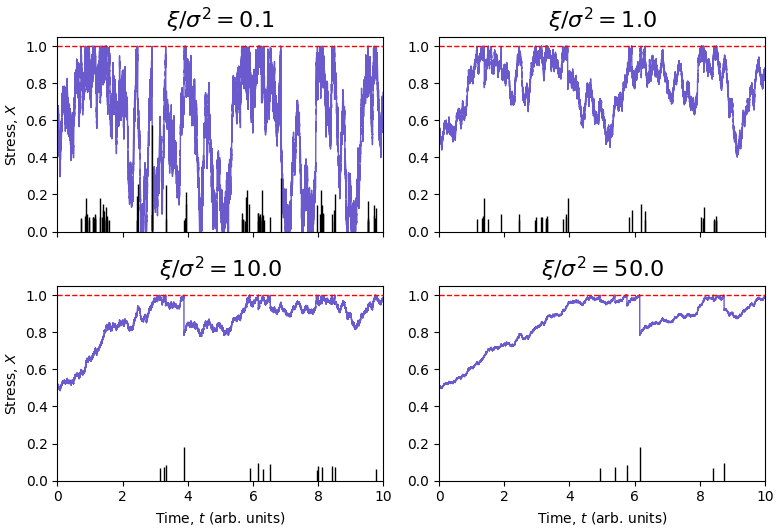
\includegraphics[width=\linewidth]{assets/traj_powerlaw.png}
        \end{minipage}%
        \hfill
        \begin{minipage}{0.47\linewidth}
            \centering
            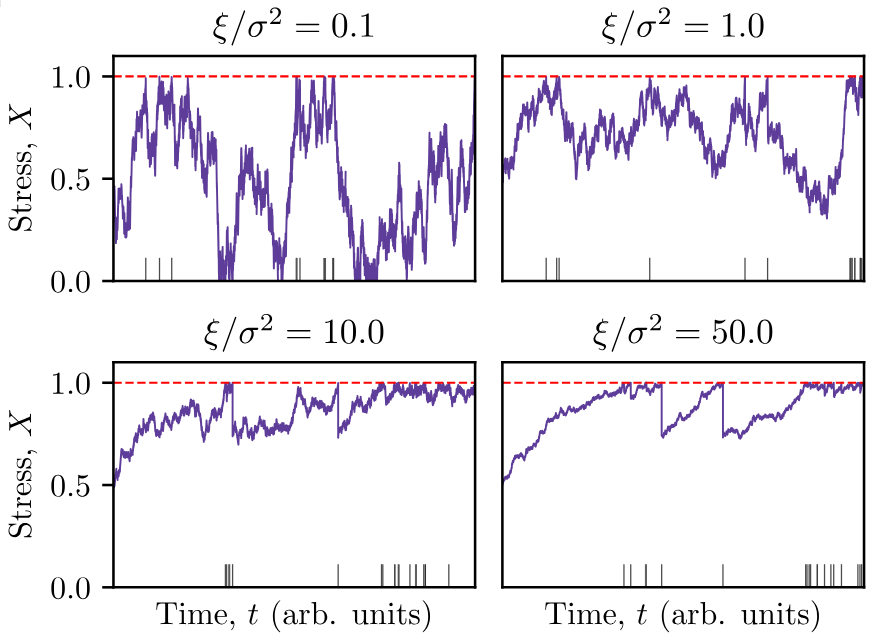
\includegraphics[width=\linewidth]{assets/traj_powerlaw_paper.png}
        \end{minipage}
        \caption{\centering Stress varying $\mu$, glitches $\sim$ power-law distribution.

        \textbf{Left}: my model, \textbf{Right}: Carlin \& Melatos (2020)}
    \end{figure}

\end{frame}

\begin{frame}{Brownian Process: other glitch sampling distribution}

    The conclusions regarding $\mu$ apply regardless of the chosen glitch size distribution.

    \begin{figure}
        \centering
        \begin{minipage}{0.49\linewidth}
            \centering
            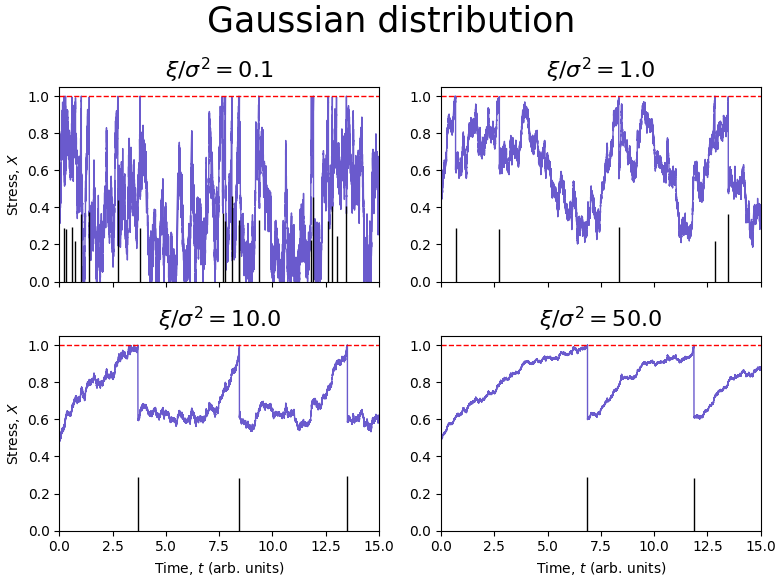
\includegraphics[width=\linewidth]{assets/traj_gaussian.png}
        \end{minipage}%
        \hfill
        \begin{minipage}{0.49\linewidth}
            \centering
            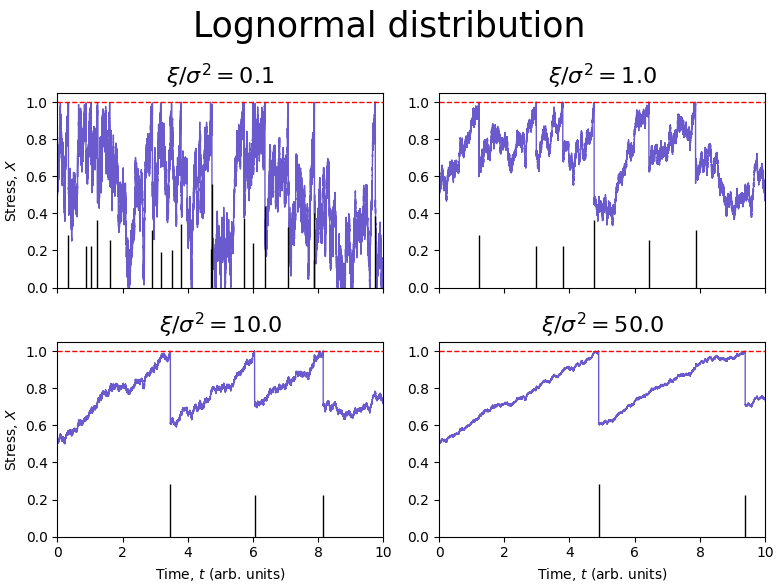
\includegraphics[width=\linewidth]{assets/traj_lognormal.png}
        \end{minipage}
        \caption{\centering Stress trajectories with different glitch size distributions:
        
        \textbf{Left}: truncated Gaussian, \textbf{Right}: truncated Lognormal.}
    \end{figure}
\end{frame}

\begin{frame}{Brownian Process: Waiting Time Distribution}
    Since the internal stress $X(t)$ is not directly observable, we focus on the statistics of glitch events:
    \begin{itemize}
        \item Waiting times between glitches, $\Delta t$.
        \item Sizes of the glitches, $\Delta X_{release}$.
    \end{itemize}
    
    \vspace{0.4cm}
    The distribution of waiting times, $p(\Delta t)$, depends on two factors:
    \begin{enumerate}
        \item \textbf{The drift/diffusion ratio $\mu$}, which controls how quickly the stress evolves towards the threshold $X_c$.
        \vspace{0.2cm}
        \item \textbf{The stress release distribution $\eta(\Delta X)$}, which sets the initial stress $X_0$ for the next interval ($X_0 \approx X_c - \Delta X_{release}$).
    \end{enumerate}
\end{frame}

\begin{frame}{Brownian Process: Waiting Time Distribution (Power-law)}
    \textbf{Power-law} glitch sizes generate a \textbf{power-law-like} waiting time distribution for low $\mu$, transitioning to \textbf{exponential-like} for high $\mu$.

    \vspace{-0.5em}

    \begin{figure}
        \centering
        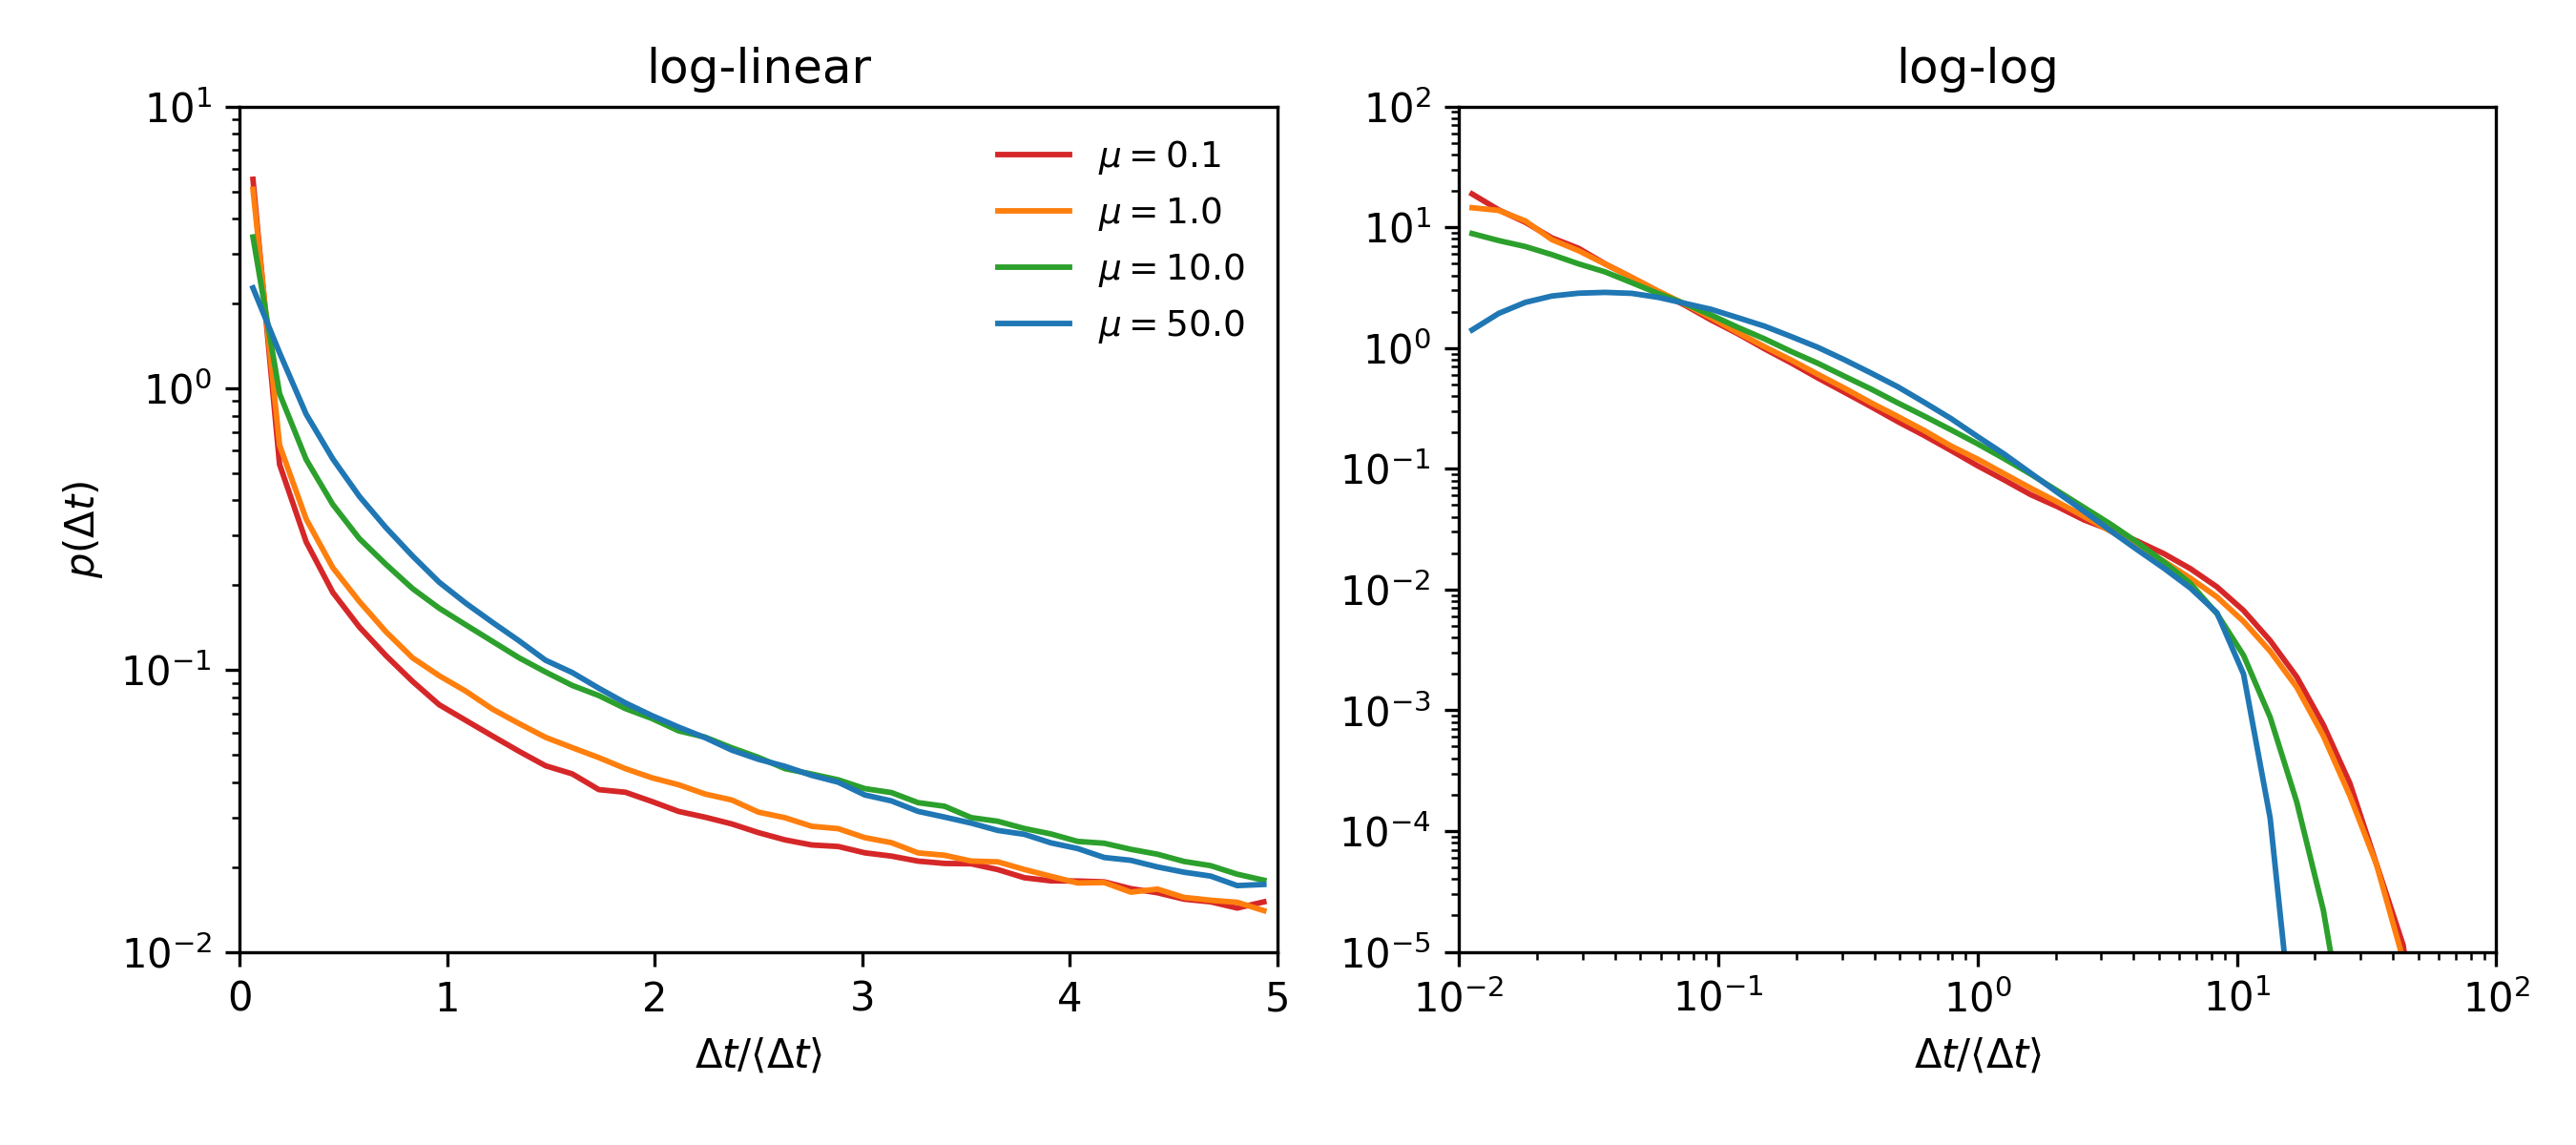
\includegraphics[width=0.52\linewidth]{assets/wtd_powerlaw.png}
        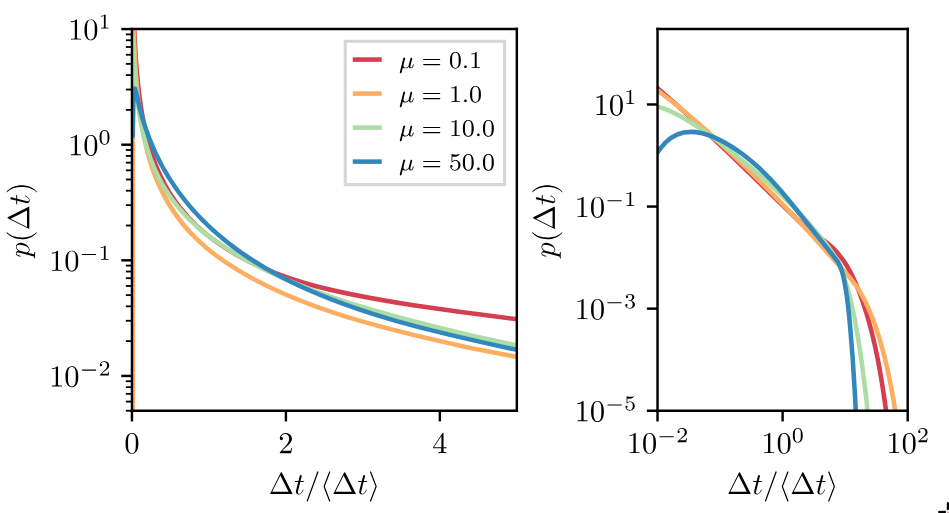
\includegraphics[width=0.52\linewidth]{assets/wtd_powerlaw_paper.png}
        \vspace{-1em}
        \caption{\centering \small $p(\Delta t)$ for glitches with power-law size distribution, varying $\mu$.
        
        \textbf{Top}: my model, \textbf{Bottom}: Carlin \& Melatos (2020)}
    \end{figure}
\end{frame}

\begin{frame}{Brownian: Waiting Time Distribution (Gaussian)}
    \setlength{\leftmargini}{0.5em}
    \small

    \vspace{-0.5em}
    \begin{itemize}
        \item \textbf{High $\mu$}: $p(\Delta t)$ is unimodal and Gaussian-like, set by the previous glitch size.
        \item \textbf{Low $\mu$}: $p(\Delta t)$ is exponential-like, dominated by random fluctuations.
    \end{itemize}

    \vspace{-1em}

    \begin{figure}
        \centering
        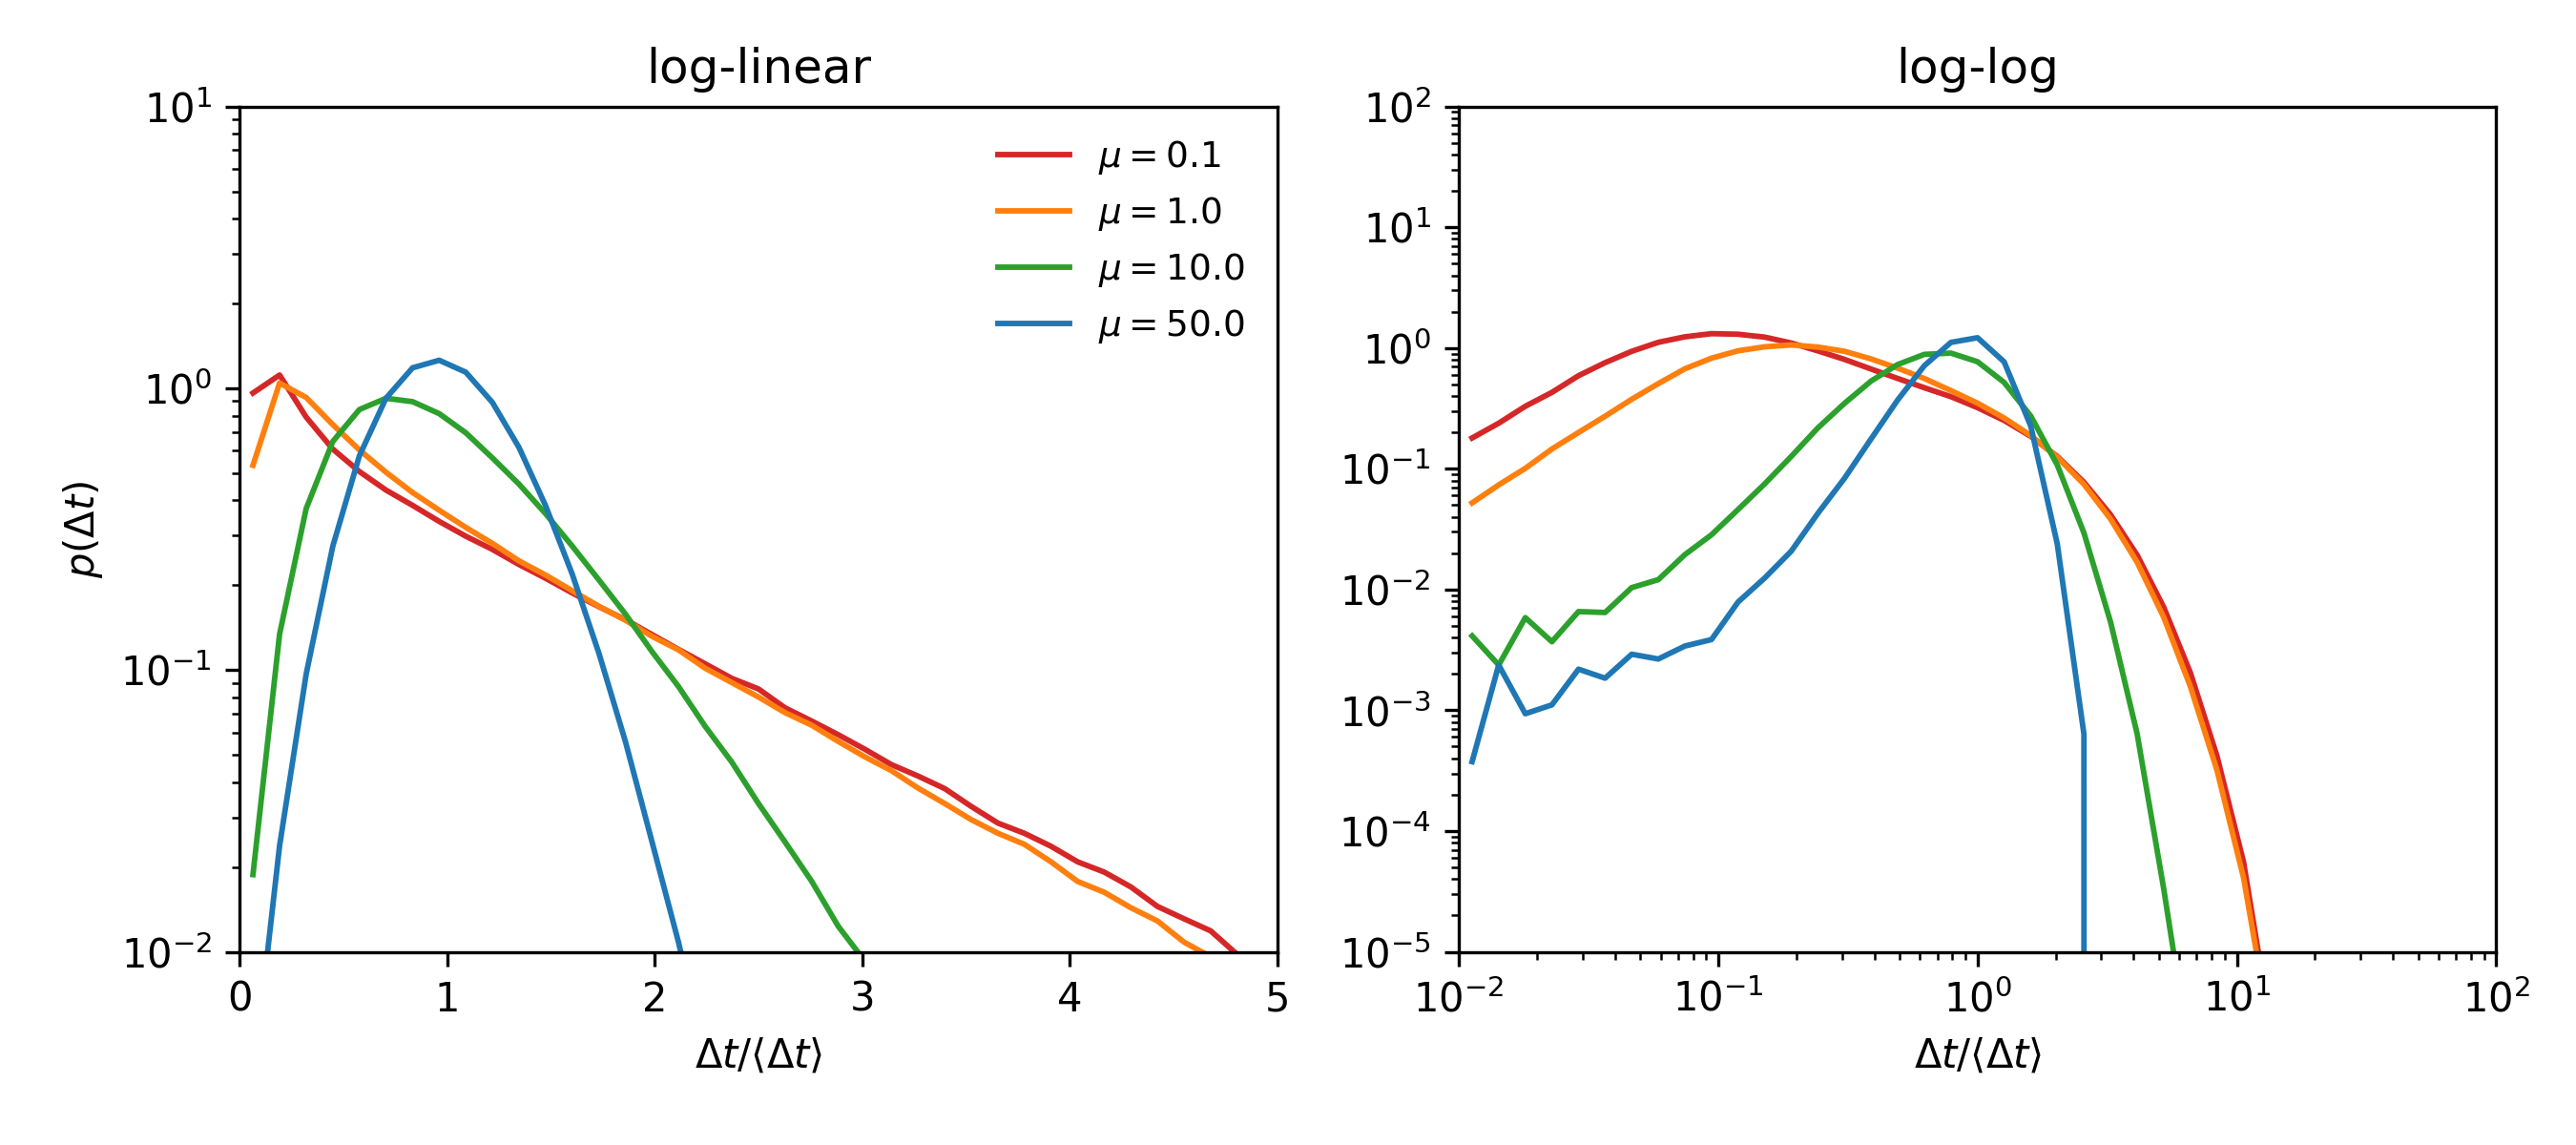
\includegraphics[width=0.52\linewidth]{assets/wtd_gaussian.png}
        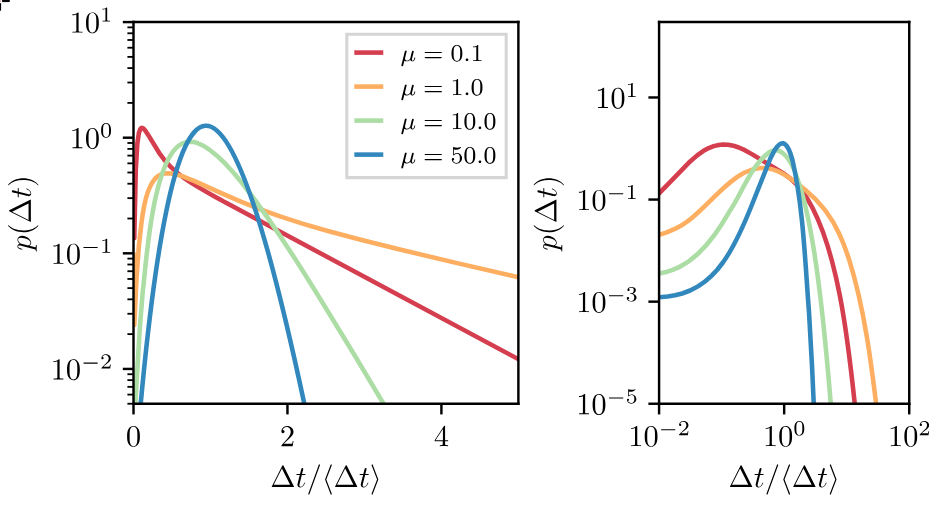
\includegraphics[width=0.52\linewidth]{assets/wtd_gaussian_paper.png}
        \vspace{-1em}
        \caption{\centering \small $p(\Delta t)$ for glitches with Gaussian size distribution, varying $\mu$.
        
        \textbf{Top}: my model, \textbf{Bottom}: Carlin \& Melatos (2020)}
    \end{figure}
\end{frame}

\begin{frame}{Brownian: Waiting Time Distribution (Lognormal)}
    \setlength{\leftmargini}{0.5em}
    \small
    \vspace{-0.5em}
    \begin{itemize}
        \item \textbf{High $\mu$}: $p(\Delta t)$ is unimodal and Gaussian-like, set by the previous glitch size.
        \item \textbf{Low $\mu$}: $p(\Delta t)$ is exponential-like, dominated by random fluctuations.
    \end{itemize}
    \vspace{-1em}
    \begin{figure}
        \centering
        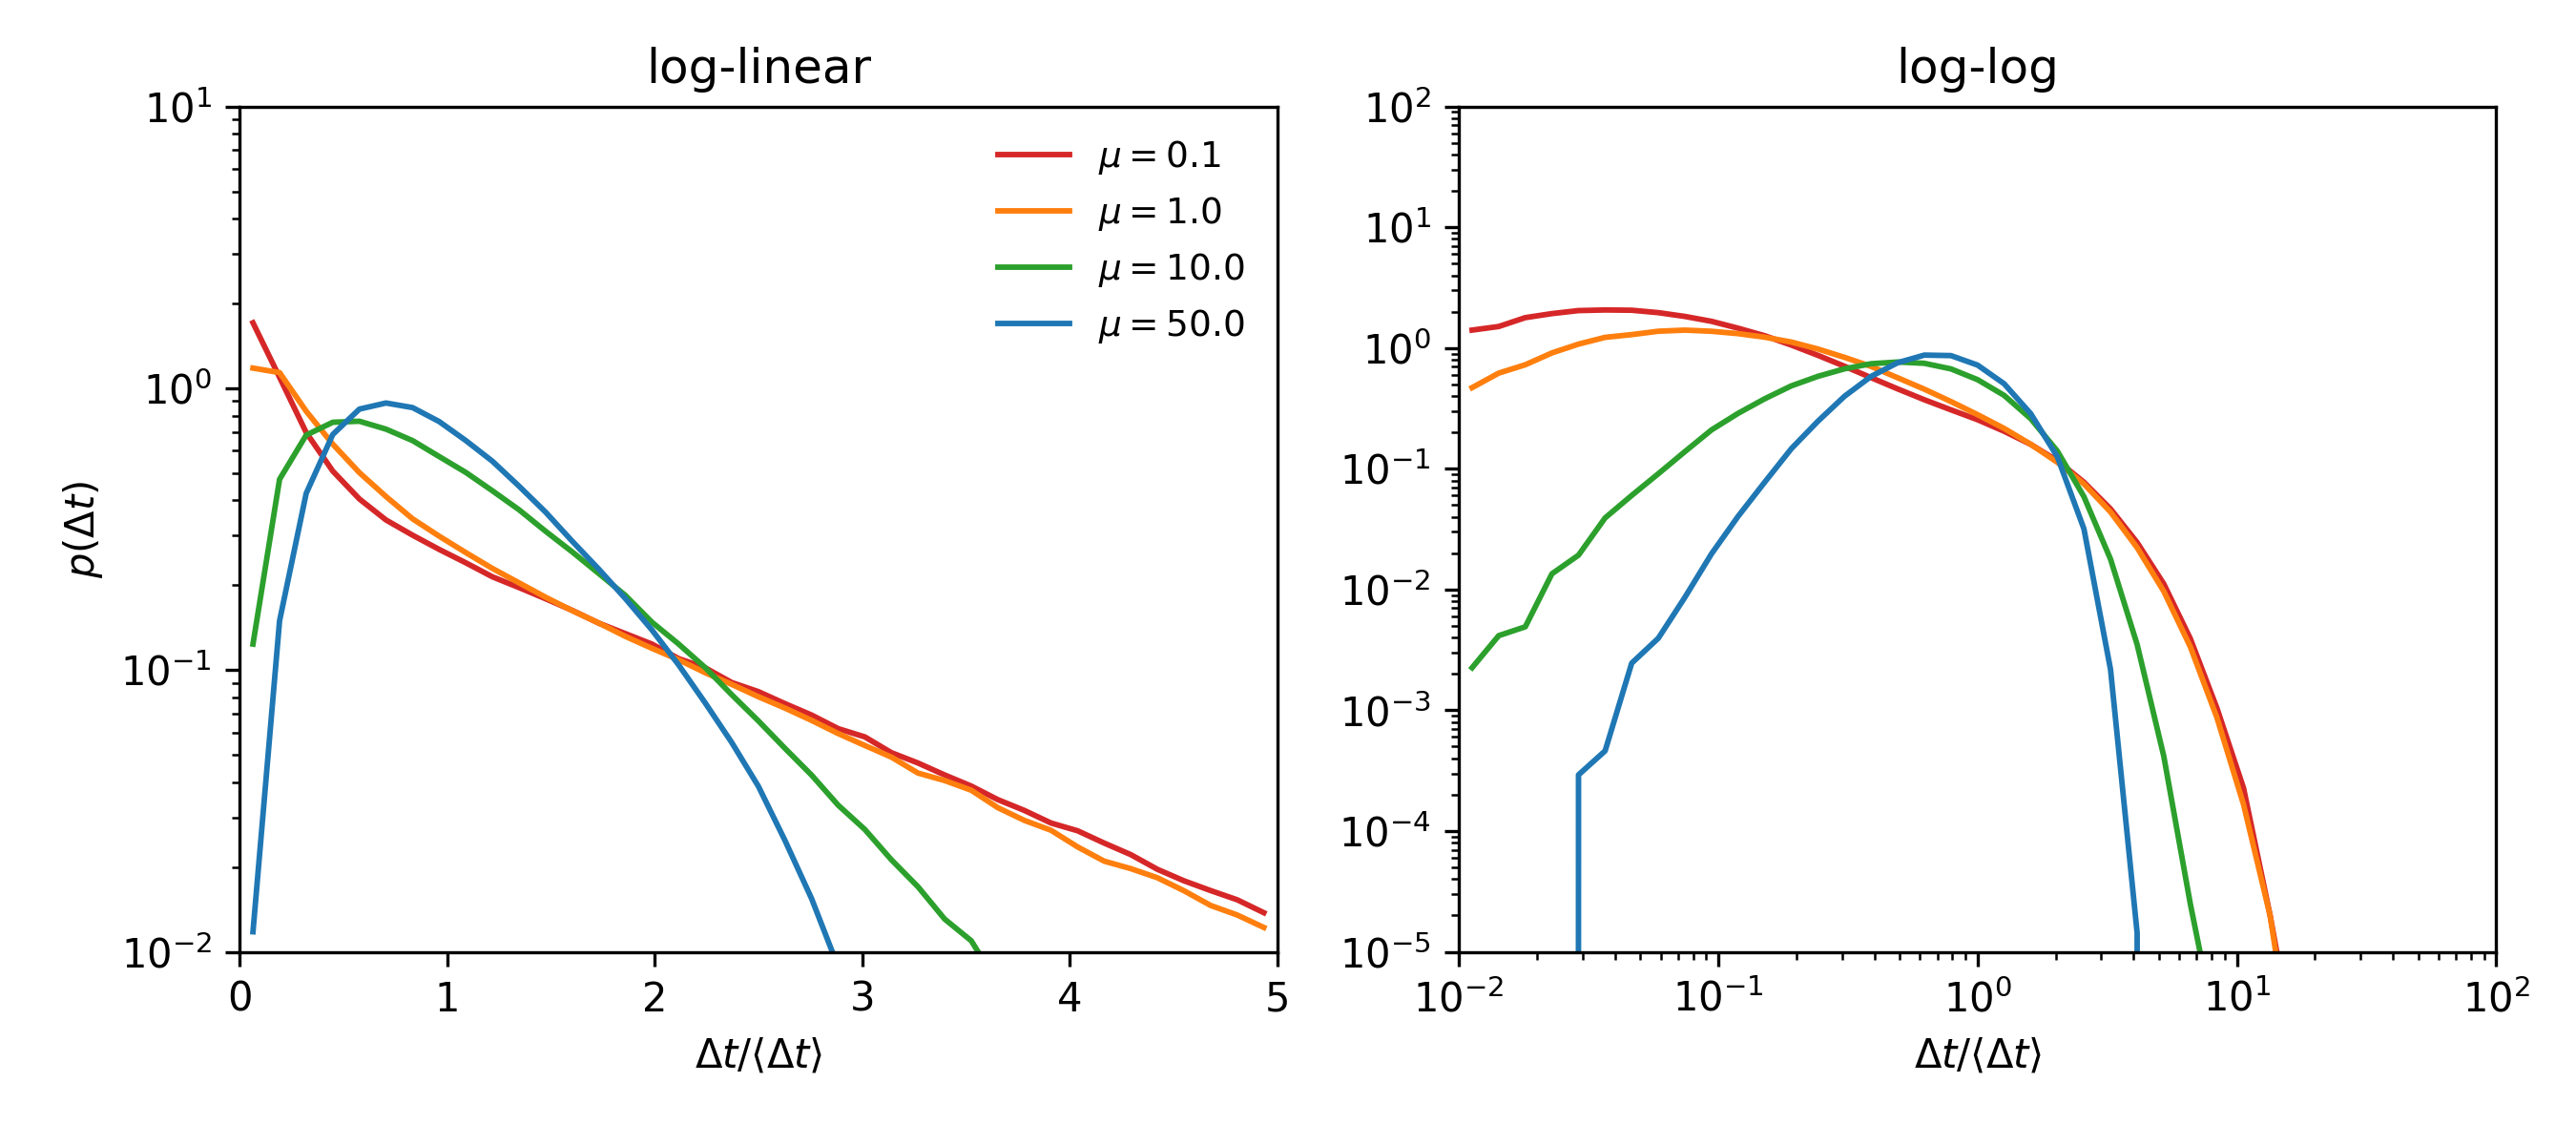
\includegraphics[width=0.52\linewidth]{assets/wtd_lognormal.png}
        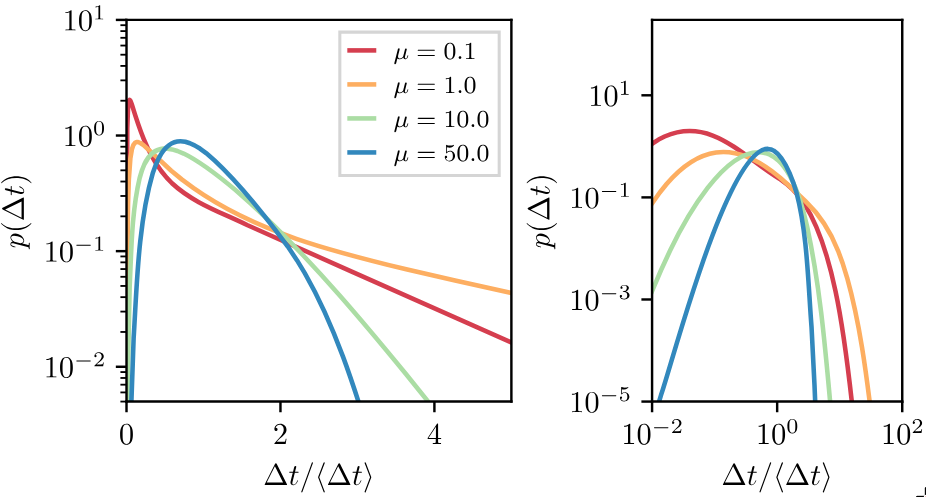
\includegraphics[width=0.52\linewidth]{assets/wtd_lognormal_paper.png}
        \vspace{-1em}
        \caption{\centering \small $p(\Delta t)$ for glitches with lognormal size distribution, varying $\mu$.
        
        \textbf{Top}: my model, \textbf{Bottom}: Carlin \& Melatos (2020)}
    \end{figure}
\end{frame}